\chapter[~]{Вивчення додаткових можливостей програми для розробки креслень sPlan}

\textbf{Мета роботи} --- ознайомитись з додатковими можливостями програми для розробки креслень схем
sPlan, навчитись працювати з формами документів, створювати власні елементи та бібліотеки
компонентів.

\section{Виконання креслення основного напису для креслення}

\begin{enumerate}[leftmargin=*]
\item Для початку роботи потрібно встановити книжну орієнтацію аркуша, та переконатись що задані
  параметри аркуша відповідають поставленому завданню. Для цього переходимо в меню ``Лист'' >
  ``Свойства листа'' (\ref{fig:lab2:document_settigns}).

  \begin{figure}[!ht]
    \centering 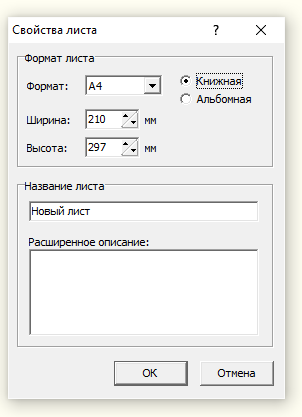
\includegraphics[]{./images/lab2/document_settings.png}
    \caption{Вікно налаштувань аркуша}
    \label{fig:lab2:document_settigns} 
  \end{figure}

  \newpage

\item Задаємо початкові розміри аркуша використовуючи інструмент
  ``Розміри'' (\ref{fig:lab2:dimentions}).
  
  \begin{figure}[!ht]
    \centering 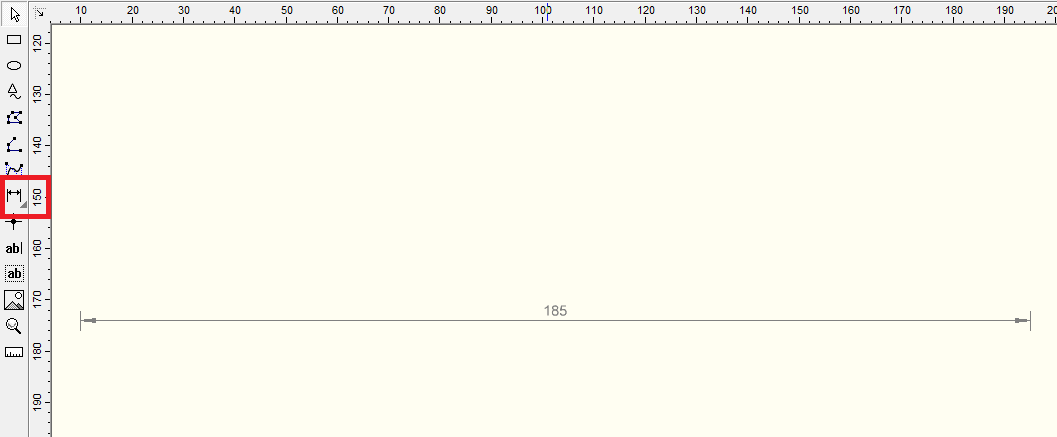
\includegraphics[width=0.9\linewidth]{./images/lab2/dimentions.png}
    \caption{Інструмент ``Розміри''}
    \label{fig:lab2:dimentions} 
  \end{figure}

\item Використовуючи інструмент ``Прямокутник'' будуємо зовнішню рамку (\ref{fig:lab2:rectangle}).
  
  \begin{figure}[!ht]
    \centering 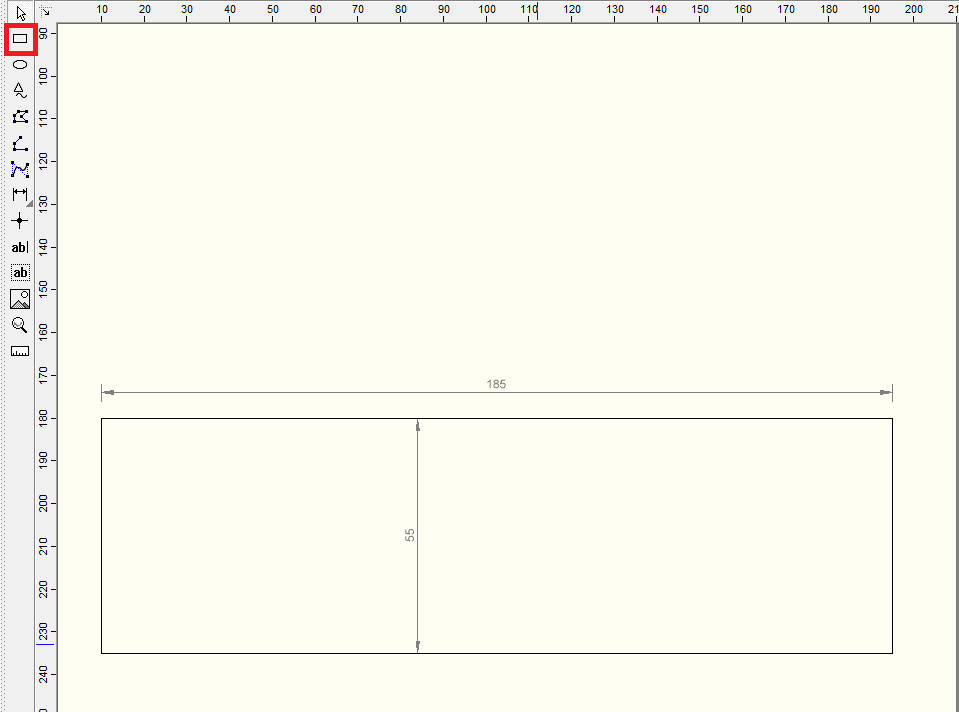
\includegraphics[width=0.9\linewidth]{./images/lab2/first_step.png}
    \caption{Інструмент ``Прямокутник''}
    \label{fig:lab2:rectangle} 
  \end{figure}

\item Використовуючи вище наведені інструменти задаємо розміри та будуємо праву частину основного
  напису (\ref{fig:lab2:rectangle}).
  
  \begin{figure}[!ht]
    \centering 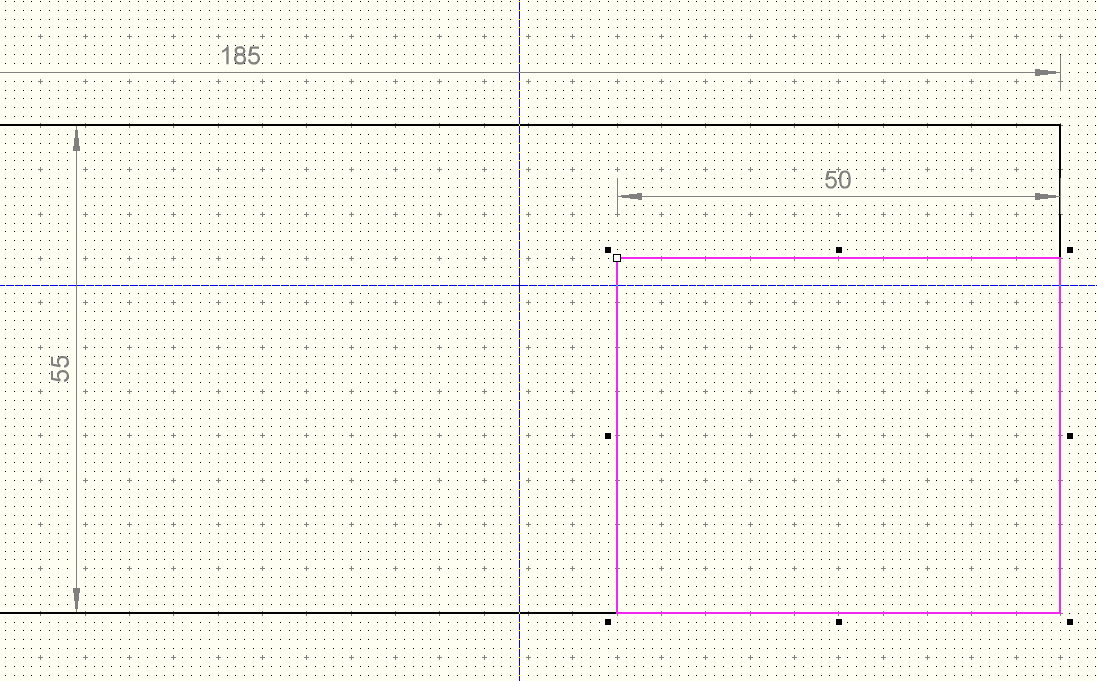
\includegraphics[width=0.9\linewidth]{./images/lab2/second_step.png}
    \caption{\label{fig:lab2:second_step}}
  \end{figure}
  \begin{figure}[!ht]
    \centering 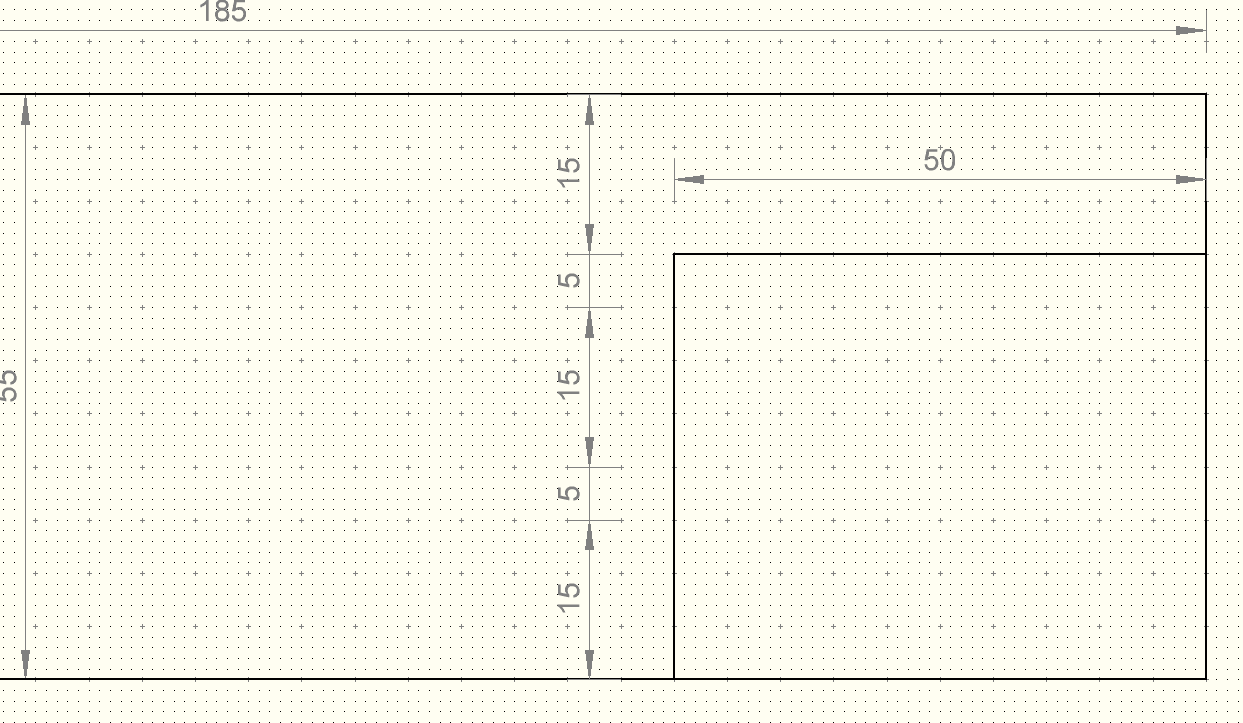
\includegraphics[width=0.9\linewidth]{./images/lab2/third_step.png}
    \caption{\label{fig:lab2:third_step}}
  \end{figure}

  \FloatBarrier

\item Застосуємо інструмент лінія, для побудови відповідних горизонтальних та вертикальних
  ліній (\ref{fig:lab2:line}).
  \begin{figure}[!htb]
    \centering 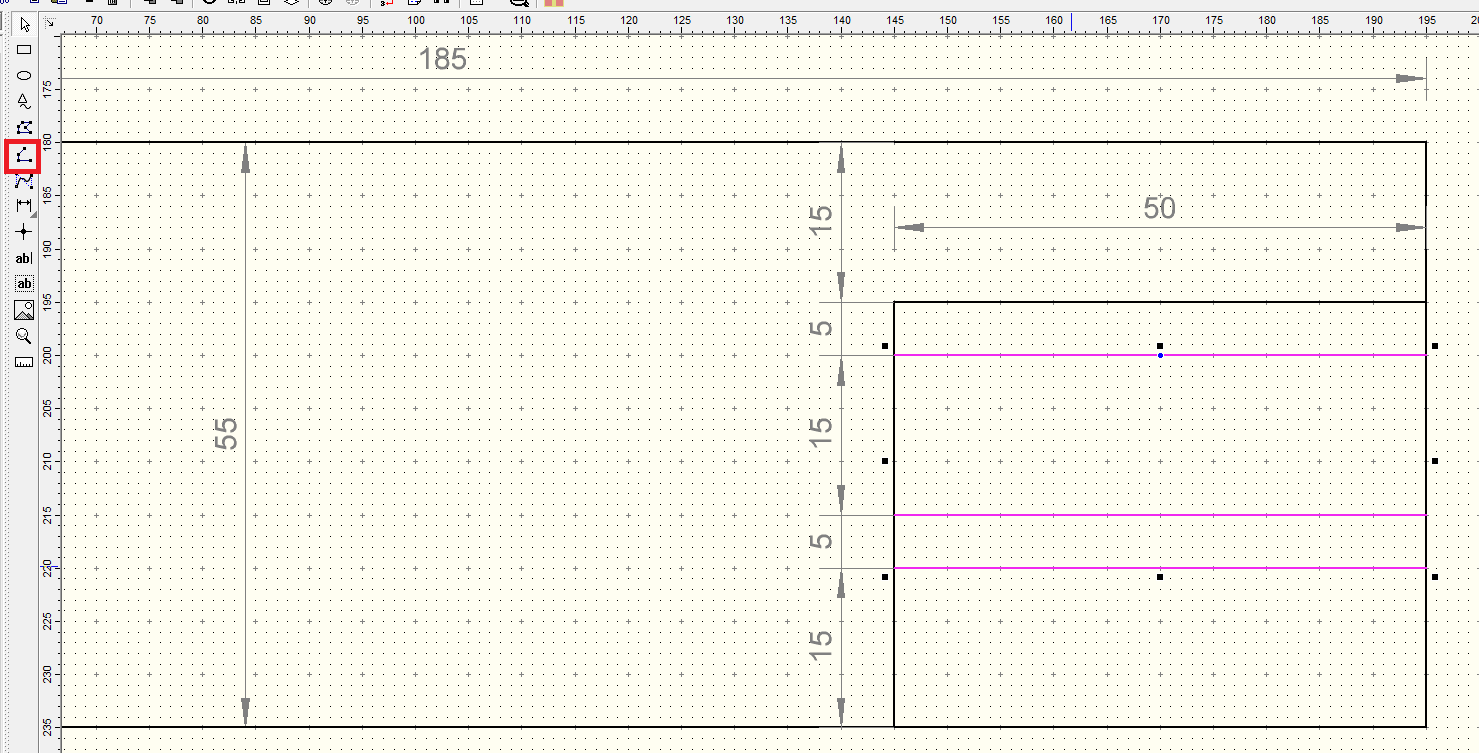
\includegraphics[width=0.9\linewidth]{./images/lab2/fourth_step.png}
    \caption{Інструмент ``Лінія''}
    \label{fig:lab2:line}
  \end{figure}
  \FloatBarrier

\item Добудовуємо залишок основного напису використовуючи вказані інструменти
  \begin{figure}[!htb]
    \centering 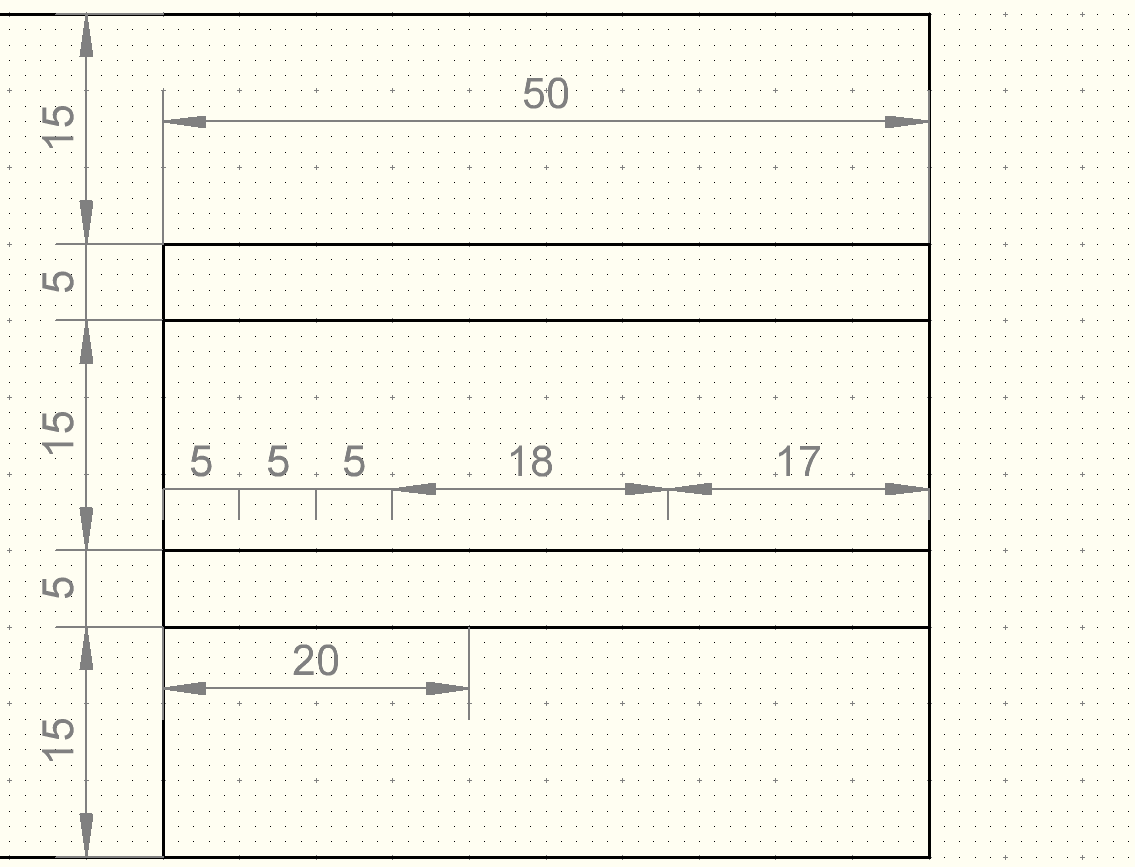
\includegraphics[width=0.9\linewidth]{./images/lab2/fifth_step.png}
    \caption{ \label{fig:lab2:fifth_step}}
  \end{figure}
  \begin{figure}[!htb]
    \centering 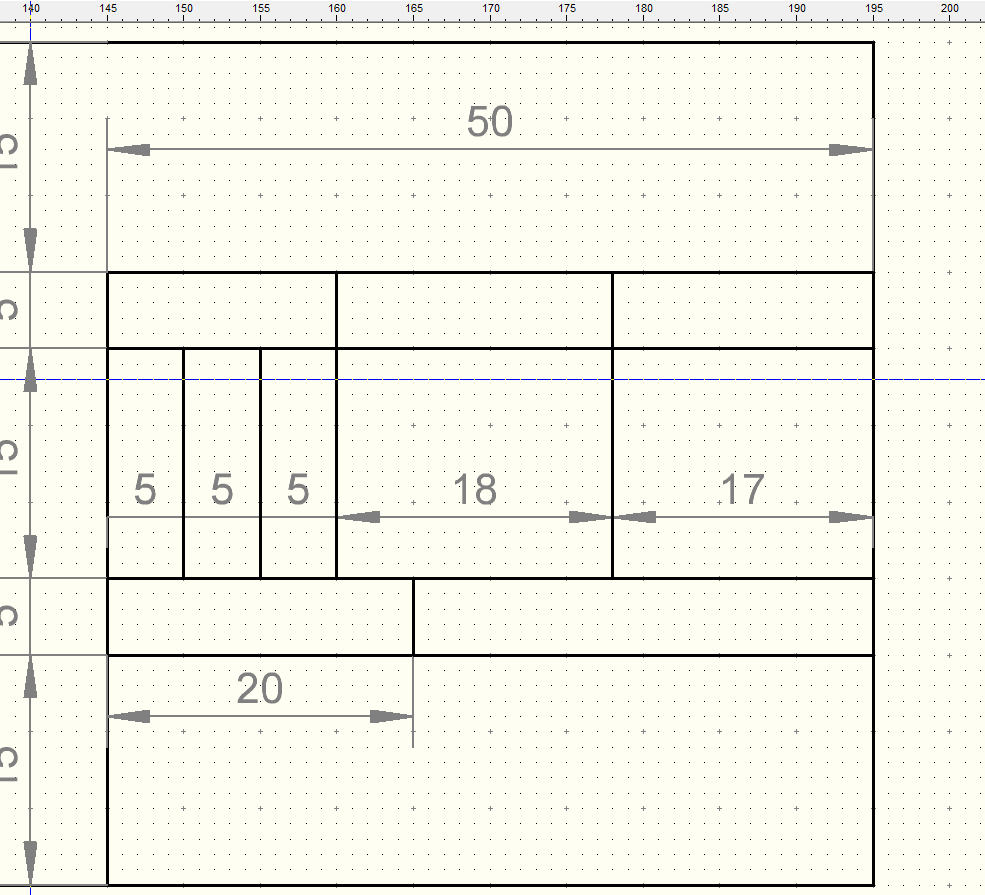
\includegraphics[width=0.9\linewidth]{./images/lab2/sixth_step.png}
    \caption{}
    \label{fig:lab2:sixth_step} 
  \end{figure}
  \begin{figure}[!htb]
    \centering 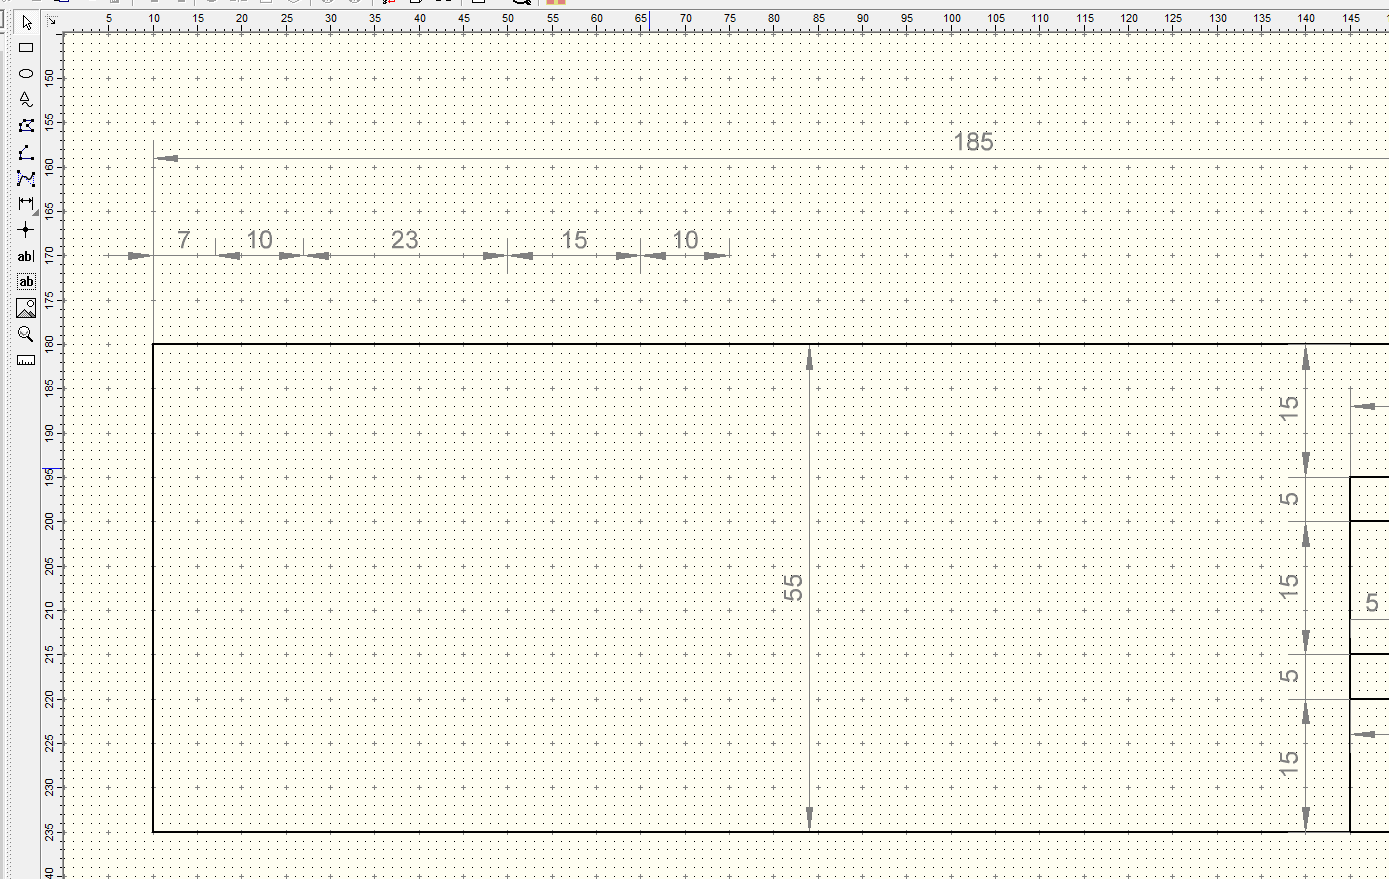
\includegraphics[width=0.9\linewidth]{./images/lab2/seventh_step.png}
    \caption{}
    \label{fig:lab2:seventh_step} 
  \end{figure}
  \begin{figure}[!htb]
    \centering 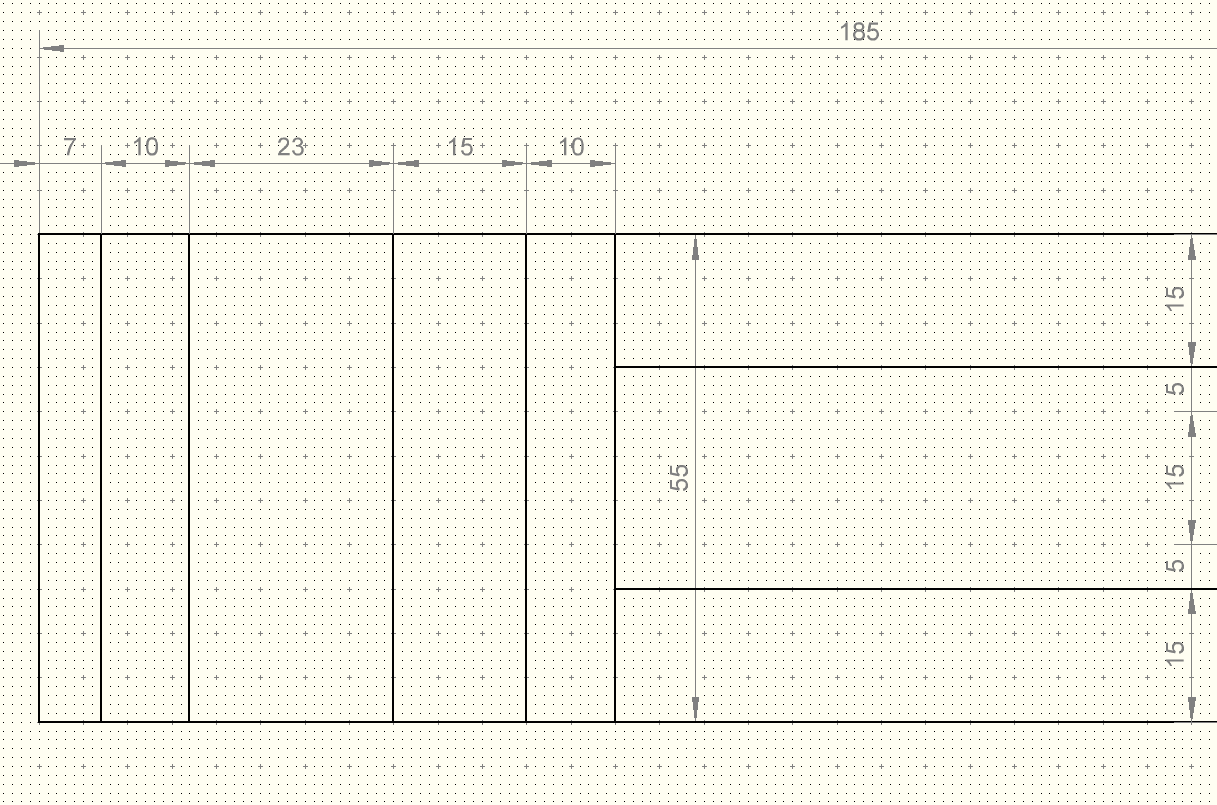
\includegraphics[width=0.9\linewidth]{./images/lab2/eighth_step.png}
    \caption{}
    \label{fig:lab2:eigth_step} 
  \end{figure}
  \begin{figure}[!htb]
    \centering 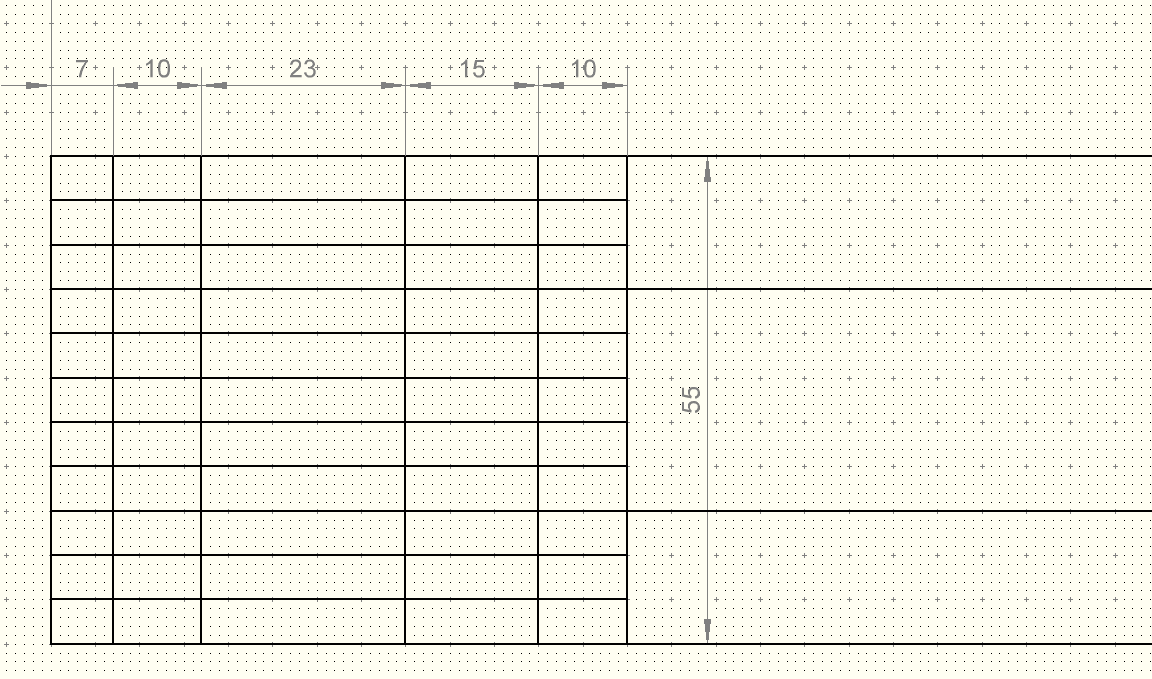
\includegraphics[width=0.9\linewidth]{./images/lab2/nineth_step.png}
    \caption{}
    \label{fig:lab2:nineth_step} 
  \end{figure}

  \FloatBarrier
\item Виділивши необхідні лінії натискаємо праву клавішу мишки та обираємо пункт ``Властивості'' в
  якому задаємо необхідну товщину лінії.
  \begin{figure}[!htb]
    \centering 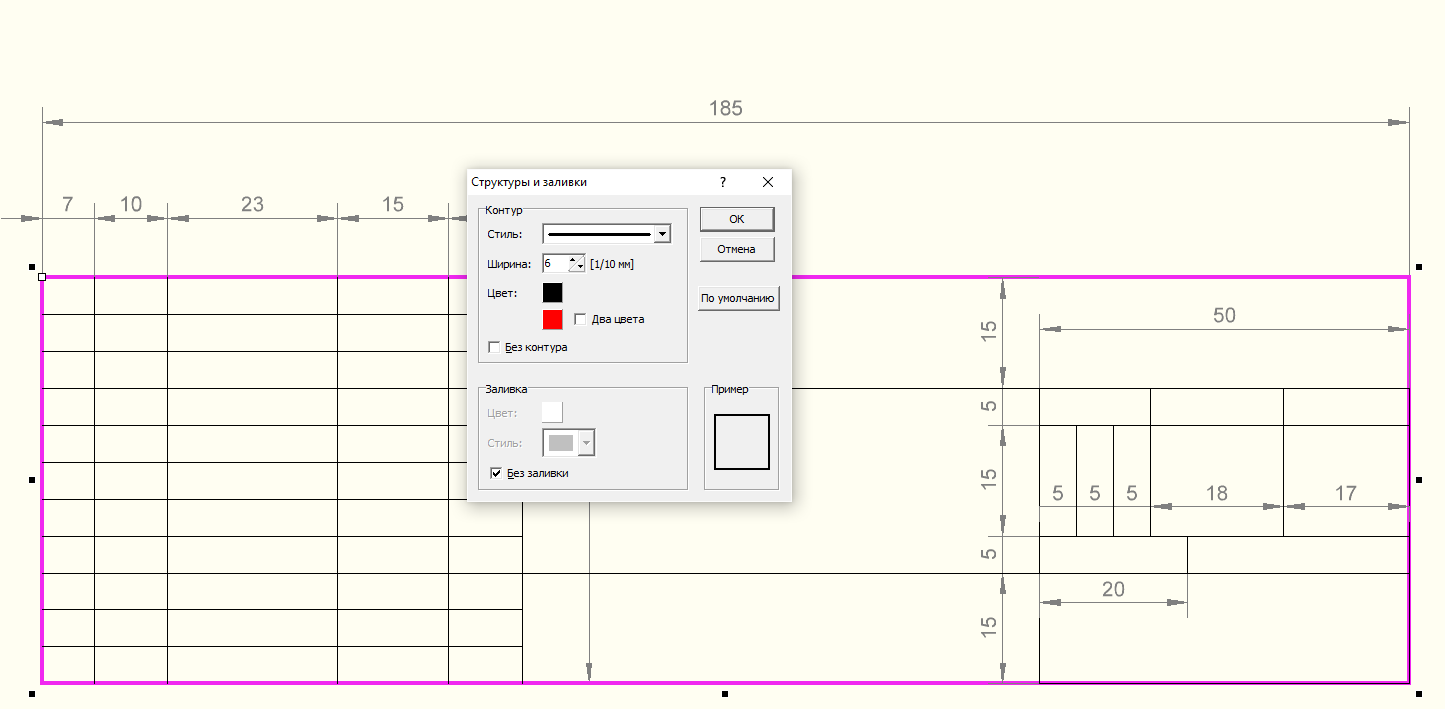
\includegraphics[width=0.9\linewidth]{./images/lab2/bold_line.png}
    \caption{}
    \label{fig:lab2:nineth_step}
  \end{figure}
  \FloatBarrier
  
\end{enumerate}

\FloatBarrier
\section{Створення користувацьої бібліотеки елементів}

Натискаємо на піктограму Книги на панелі бібліотек і обираємо пункт ``Бібліотеки...''. У діалоговому
віні обираємо пункт ``Створити'' (\ref{fig:lab2:create_library}).
\begin{figure}[!htb]
  \centering 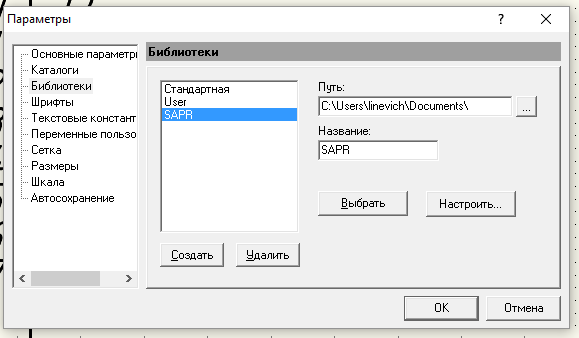
\includegraphics[width=0.9\linewidth]{./images/lab2/new_library.png}
  \caption{Вікно керування бібліотеками.}
  \label{fig:lab2:create_library}
\end{figure}
\FloatBarrier

\section{Виконання крелсення елементів електронної схеми за варіантом}

Згідно варіанту портрібно створити наступні елементи:
\begin{figure}[!htb]
  \begin{subfigure}[b]{.4\linewidth}
    \centering 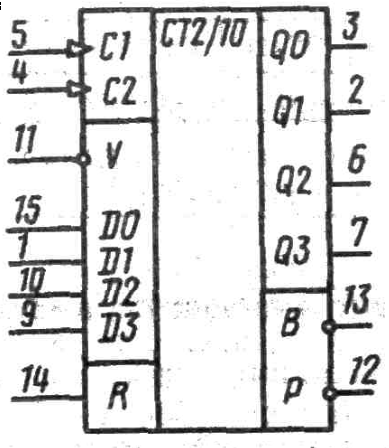
\includegraphics[width=.8\linewidth]{./images/lab2/target_element1.png}
    \caption{К555ИЕ6}
    \label{fig:lab2:target_element1}
  \end{subfigure}
  \hfill
  \begin{subfigure}[b]{.4\linewidth}
    \centering 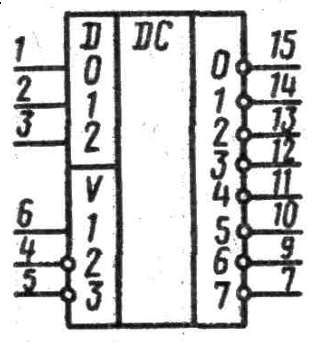
\includegraphics[width=.8\linewidth]{./images/lab2/target_element2.png}
    \caption{К555ИД7}
    \label{fig:lab2:target_element2}
  \end{subfigure}
  \caption{\label{fig:lab2:target_elements}}
\end{figure}
\FloatBarrier

Для створення елементів в бібліотеці на панелі клікаємо правою клавішою мишки, у випадаючому меню
обираємо ``Створити новий елемент'' > ``Редактор''. У відкритому вікні створюємо необхідні елементи.

\begin{enumerate}[leftmargin=*]
\item За домогою стандартних примітивів креслимо задані елементи (\ref{fig:lab2:element1_step1}).
  \begin{figure}[!htb]
    \centering 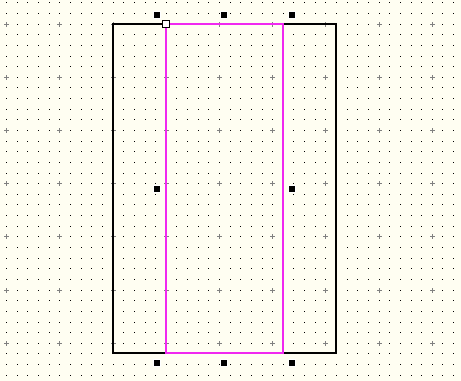
\includegraphics[width=0.6\linewidth]{./images/lab2/element1_step1.png}
    \caption{\label{fig:lab2:element1_step1}}
  \end{figure}
  \FloatBarrier
\item Задаємо заливку для необхідних елементів (\ref{fig:lab2:element1_step2}).
  \begin{figure}[!htb]
    \centering 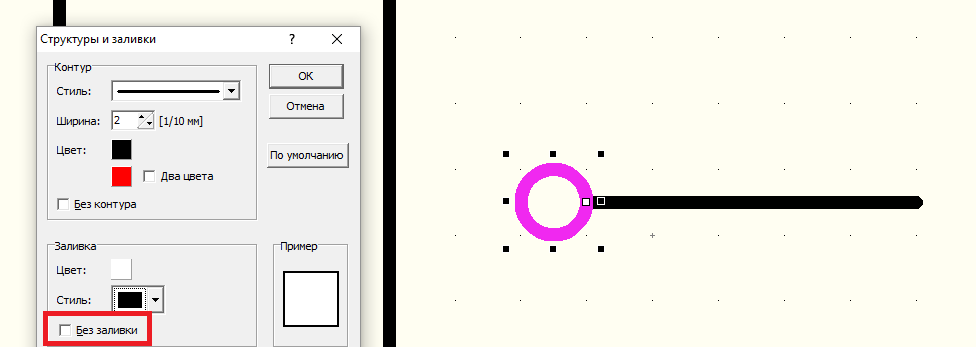
\includegraphics[width=0.9\linewidth]{./images/lab2/element1_step2.png}
    \caption{\label{fig:lab2:element1_step2}}
  \end{figure}
  \FloatBarrier
\item Створюємо підписи до контактів та інші необхідні текстові елементи
  (\ref{fig:lab2:element1_step3}).
  \begin{figure}[!htb]
    \centering 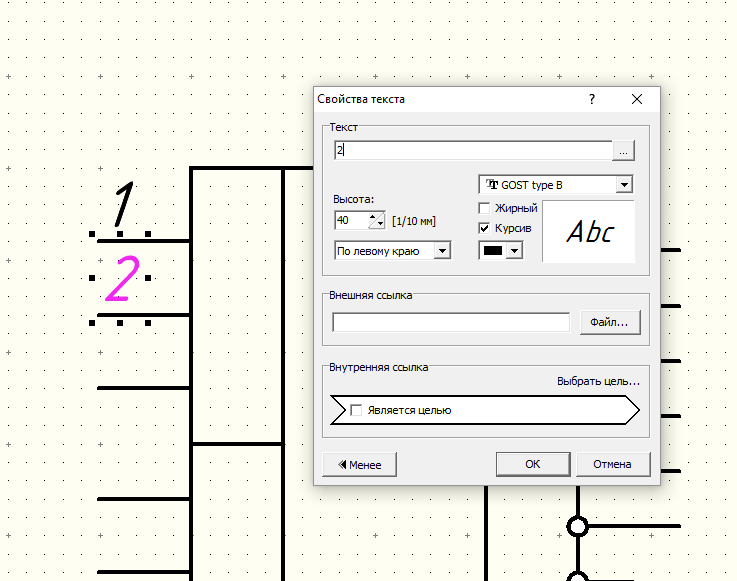
\includegraphics[width=0.9\linewidth]{./images/lab2/element1_step3.png}
    \caption{\label{fig:lab2:element1_step3}}
  \end{figure}
  \FloatBarrier
\item Аналогічно вибудовуємо другий елемент (\ref{fig:lab2:element2}).
  \begin{figure}[!htb]
    \centering 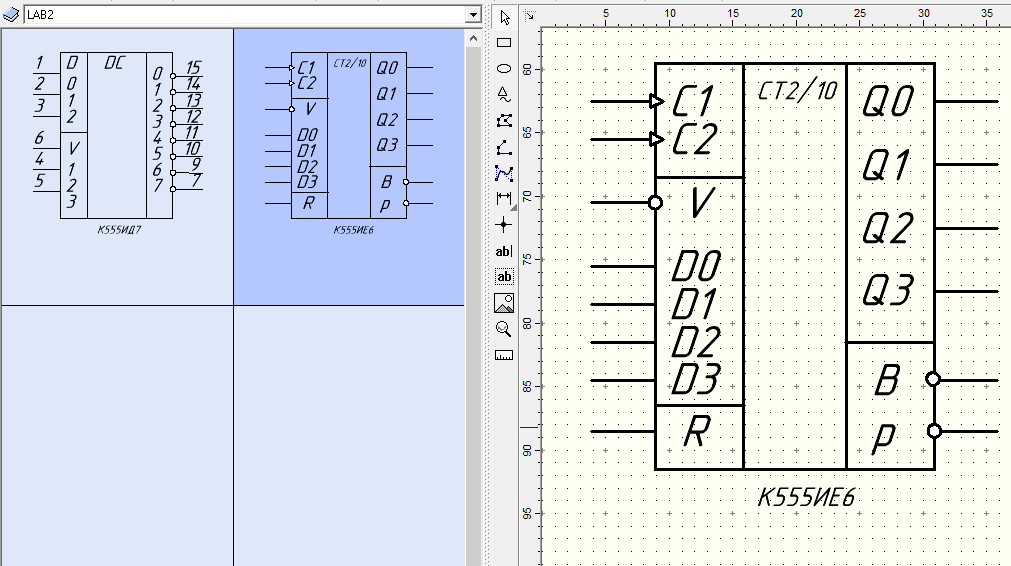
\includegraphics[width=0.9\linewidth]{./images/lab2/element2.png}
    \caption{Готові елементи в бібліотеці}
    \label{fig:lab2:element2}
  \end{figure}
  \FloatBarrier
\end{enumerate}



\section{Виконання креслення електронної принципової схеми з використанням створених елементів}

\section{Створення переліку  елементів схеми}

